

\newpage

%----------------------------------------------------------------------------------------


%\section[Static User Equilibrium][Equilibre Utilisateur Statique]{Investigating the Empirical Existence of Static User Equilibrium}{Investigation Empirique de l'Existence de l'Equilibre Utilisateur Statique}

\section{Static User Equilibrium}{Equilibre Utilisateur Statique}


\label{sec:transportationequilibrium}



%----------------------------------------------------------------------------------------


\bpar{
The Static User Equilibrium is a powerful framework for the theoretical study of traffic. Despite the restricting assumption of stationary flows that intuitively limit its application to real traffic systems, many operational models implementing it are still used without an empirical validation of the existence of the equilibrium. We investigate its existence on a traffic dataset of three months for the region of Paris, FR. The implementation of an application for interactive spatio-temporal data exploration allows to hypothesize a high spatial and temporal heterogeneity, and to guide further quantitative work. The assumption of locally stationary flows is invalidated in a first approximation by empirical results, as shown by a strong spatial and temporal variability in shortest paths and in network topological measures such as betweenness centrality. Furthermore, the behavior of spatial autocorrelation index of congestion patterns at different spatial ranges suggest a chaotic evolution at the local scale, especially during peak hours. We finally discuss the implications of these empirical findings and describe further possible developments based on the estimation of Lyapunov dynamical stability of traffic flows.
}{
L'Equilibre Utilisateur Statique est un cadre puissant pour l'étude théorique du trafic. Malgré l'hypothèse restreignante\comment[FL]{de quel point de vue ?} de stationnarité des flots qui intuitivement limite son application aux systèmes de trafic réels, de nombreux modèles opérationnels qui l'implémentent sont toujours utilisés sans validation empirique de l'existence de l'équilibre. Nous étudions celle-ci sur un jeu de données de trafic couvrant trois mois sur la région parisienne. L'implémentation d'une application d'exploration interactive de données spatio-temporelles permet de formuler l'hypothèse d'une forte hétérogénéité spatiale et temporelle, guidant les études quantitatives. L'hypothèse de flots localement stationnaires est invalidée en première approximation par les résultats empiriques, comme le montrent une forte variabilité spatio-temporelle des plus courts chemins et des mesures topologiques du réseau comme la centralité de chemin. De plus, le comportement de l'index d'autocorrelation spatiale pour les motifs de congestion à différentes portées spatiales suggère une évolution chaotique à l'échelle locale, en particulier lors des heures de pointe. Nous discutons finalement les implications de ces résultats empiriques et proposons des possibles développements futurs basés sur l'estimation de la stabilité dynamique au sens de Lyapounov des flots de trafic.
}


%%%%%%%%%%%%%%%%%%%%%%%
\subsection{Context}{Contexte}
\label{treq:introduction}


\bpar{
Traffic Modeling has been extensively studied since seminal work by~\cite{wardrop1952road} : economical and technical elements at stake justify the need for a fine understanding of mechanisms ruling traffic flows at different scales. Many approaches with different purposes coexist today, of which we can cite dynamical micro-simulation models, generally opposed to equilibrium-based techniques. Whereas the validity of micro-based models has been largely discussed and their application often questioned, the literature is relatively poor on empirical studies assessing the stationary equilibrium assumption in the Static User Equilibrium (SUE) framework. Various more realistic developments have been documented in the literature, such as Dynamic Stochastic User Equilibrium (DSUE) (see e.g. a description by~\cite{han2003dynamic}). An intermediate between static and stochastic frameworks is the Restricted Stochastic User Equilibrium, for which route choice sets are constrained to be realistic (\cite{rasmussen2015stochastic}). Extensions that incorporate user behavior with choice models have more recently been proposed, such as~\cite{zhang2013dynamic} taking into account both the influence of road pricing and congestion on user choice with a Probit model. Relaxations of other restricting assumptions such as pure user utility maximization have been also introduced, such as the Boundedly Rational User Equilibrium described by~\cite{mahmassani1987boundedly}. In this framework, user have a range of satisfying utilities and equilibrium is achieved when all users are satisfied. It produces more complex features such as the existence of multiple equilibria, and allows to account for specific stylized facts such as irreversible network change as developed by~\cite{guo2011bounded}. Other models for traffic assignment, inspired from other fields have also recently been proposed : in~\cite{puzis2013augmented}, an extended definition of betweenness centrality combining linearly free-flow betweenness with travel-time weighted betweenness yield a high correlation with effective traffic flows, acting thus as a traffic assignment model. It provides direct practical applications such as the optimization of traffic monitors spatial distribution.
}{
La modélisation du trafic a été largement étudiée depuis les travaux séminaux de Wardrop (\cite{wardrop1952road}) : les enjeux économiques et techniques justifient entre autre le besoin d'une compréhension fine des mécanismes régissant les flots de trafic à différentes échelles. Différentes approches aux objectifs différents coexistent aujourd'hui, parmi lesquels on trouve par exemple les modèles dynamiques de micro-simulation, généralement opposés aux techniques de basant sur l'équilibre. Tandis que la validité des modèles microscopiques a été étudiée de façon conséquente et leur application souvent questionnée, la littérature est relativement pauvre en études empiriques assurant l'hypothèse d'équilibre stationnaire du cadre de l'Equilibre Utilisateur Statique (EUS). De nombreux développements plus réalistes on été documentés dans la littérature, tels l'Equilibre Utilisateur Dynamique Stochastique (EUDS) (voir pour une description par example~\cite{han2003dynamic}). A un niveau intermédiaire entre les cadres statiques et stochastiques se trouve l'Equilibre Utilisateur Stochastique Restreint, pour lequel les choix d'itinéraire des utilisateurs sont contraints à un ensemble d'alternatives réalistes (\cite{rasmussen2015stochastic}). D'autres extensions prenant en compte le comportement de l'utilisateur via des modèles de choix ont été proposé plus récemment, comme~\cite{zhang2013dynamic} qui inclut à la fois l'influence de la tarification routière et de la congestion sur le choix avec un modèle Probit. La relaxation d'autres hypothèses restrictives comme la maximisation pure de l'utilité par l'utilisateur ont aussi été introduites, tels l'Equilibre Utilisateur Borné décrit par~\cite{mahmassani1987boundedly}. Dans ce cadre, l'utilisateur est satisfait si son utilité tombe dans un intervalle et l'équilibre est achevé lorsque chaque utilisateur est satisfait. Les dynamiques résultantes sont plus complexes comme révélé par l'existence d'équilibres multiples, et permet de rendre compte de faits stylisés spécifiques comme des évolutions irréversibles du réseau comme développé par~\cite{guo2011bounded}. D'autres modèles d'attribution de trafic inspirés d'autres domaines ont également été plus récemment proposés: dans~\cite{puzis2013augmented}, une définition étendue de la centralité de chemin qui combine linéairement le centralité des flots non-contraints avec une centralité pondérée par le temps de parcours permet d'obtenir une forte corrélation avec les flots de trafic effectifs, fournissant ainsi un modèle d'attribution de trafic. Cela fournit également des applications pratiques comme l'optimisation de la distribution spatiale des capteurs de trafic.
}

\bpar{
Despite all these developments, some studies and real-world applications still rely on Static User Equilibrium. Parisian region e.g. uses a static model (MODUS) for traffic management and planning purposes. \cite{leurent2014user} introduce a static model of traffic flow including parking cruising and parking lot choice: it is legitimate to ask, specifically at such small scales, if the stationary distribution of flows is a reality. An example of empirical investigation of classical assumptions is given in~\cite{zhu2010people}, in which revealed route choices are studied. Their conclusions question ``Wardrop’s first principle'' implying that users choose among a well-known set of alternatives. In the same spirit, we investigate the possible existence of the equilibrium in practice. More precisely, SUE assumes a stationary distribution of flows over the whole network. This assumption stays valid in the case of local stationarity, as soon as time scale for parameter evolution is considerably greater than typical time scales for travel. The second case which is more plausible and furthermore compatible with dynamical theoretical frameworks, is here tested empirically. 
}{
Malgré ces nombreux développements, de nombreuses études et applications concrètes se reposent toujours\comment[FL]{?} sur l'Equilibre Utilisateur Statique. La région parisienne utilise par exemple un modèle statique (MODUS) pour gérer et planifier le trafic. \cite{leurent2014user} introduit un modèle statique de flots qui inclut les recherches locales et le choix du parking : il est légitime de s'interroger, en particulier à de si faibles échelles, si la stationnarité de la distribution des flots est une réalité. Une example d'exploration empirique des hypothèses classiques est donné par~\cite{zhu2010people}, pour lequel les choix d'itinéraires révélés sont étudiés. Les conclusions questionnent le ``premier principe de Wardrop'' qui implique que les utilisateurs choisissent parmi un ensemble d'alternatives parfaitement connu. Dans le même esprit, nous étudions l'existence possible de l'équilibre en pratique. Plus précisément, l'EUS suppose une distribution stationnaire des flots sur l'ensemble du réseau. Cette hypothèse reste valable dans le cas d'une stationnarité locale, tant que l'échelle temporelle d'évolution des paramètres est considérablement plus grande que les échelles typiques de voyage. Le second cas qui est plus plausible et de plus compatible avec les cadres théoriques dynamiques est testé ici.\comment[FL]{smt (?) : tu ne dis pas ce que tu veux faire ni pourquoi.}
}


\bpar{
The rest of the paper is organized as follows : data collection procedure and dataset are described ; we present then an interactive application for the interactive exploration of the dataset aimed to give intuitive insights into data patterns ; we present then results of various quantitative analyses that give convergent evidence for the non-stationarity of traffic flows ; we finally discuss implications of these results and possible developments.
}{
La suite de ce travail s'organise ainsi : la procédure de collection de données ainsi que le jeu de données sont décrits ; nous présentons ensuite une application interactive pour l'exploration du jeu de données, dans le but de fournir une intuitions sur les motifs présents ; puis nous donnons divers résultats d'analyses quantitatives allant dans le sens d'indices convergents pour une non-stationnarité des flots de trafic ; nous discutons finalement les implications de ces résultats et des développements possibles.
}



%%%%%%%%%%%%%%%%%%%%%
\subsection{Results}{Résultats}


%%%%%%%%%%%%%%%%%%%%%
\subsubsection{Data collection}{Collecte des données}

%%%%%%%%%%%%%%%%%%%%%
\paragraph{Dataset Construction}{Construction du jeu de données}


\bpar{
We propose to work on the case study of Parisian Metropolitan Region. An open dataset was constructed for highway links within the region, collecting public real-time open data for travel times (available at www.sytadin.fr). As stated by~\cite{bouteiller2013open}, the availability of open datasets for transportation is far to be the rule, and we contribute thus to a data opening by the construction of our dataset. Our data collection procedure consists in the following simple steps, executed each two minutes by a \texttt{python} script :
\begin{itemize}
\item fetch raw webpage giving traffic information
\item parse html code to retrieve traffic links id and their corresponding travel time
\item insert all links in a \texttt{sqlite} database with the current timestamp.
\end{itemize}
}{
Nous proposons de travailler sur l'étude de cas de la région métropolitaine de Paris. Un jeu de données ouvert\comment[FL]{as tu le droit de l'ouvrir ?}[(JR) je le prends] a été construit, comprenant les liens autoroutiers dans la région, par collecte des données publiques en temps réel des temps de parcours (disponible sur www.sytadin.fr). Comme rappelé par~\cite{bouteiller2013open}, la disponibilité de jeux de données ouverts pour les transports est loin d'être la règle, et nous contribuons ainsi à une ouverture par la construction de notre jeu de données. La procédure de collecte de données consiste en les points suivants, executés toutes les deux minutes par un script \texttt{python} :
\begin{itemize}
\item récupération de la page web brute donnant les informations de trafic
\item parsing du code html afin de récupérer les identifiants des liens de trafic et les temps de parcours correspondants
\item insertion des liens dans une base \texttt{sqlite} avec le temps courant.
\end{itemize}
}


\bpar{
The automatized data collection script continues to enrich the database as time passes, allowing future extensions of this work on a larger dataset and a potential reuse by scientists or planners. The latest version of the dataset is available online (sqlite format) under a Creative Commons License\footnote{at \texttt{http://37.187.242.99/files/public/sytadin{\_}latest.sqlite3}}.
}{
Le script automatisé de collection des données continue d'enrichir la base au fur et à mesure du temps, permettant des développements futurs de ce travail sur un jeu de données plus large, et une réutilisation potentielle pour des travaux scientifiques ou opérationnels. La dernière version du jeu de données au format sqlite est disponible en ligne sous une Licence \emph{Creative Commons}\footnote{à l'adresse \texttt{http://37.187.242.99/files/public/sytadin{\_}latest.sqlite3}}.
}


%%%%%%%%%%%%%%%%%%%%%
\paragraph{Data Summary}{Description des données}


\bpar{
A time granularity of 2 minutes was obtained for a three months period (February 2016 to April 2016 included). Spatial granularity is in average 10km, as travel times are provided for major links. The dataset contains 101 links. Raw data we use is effective travel time, from which we can construct travel speed and relative travel speed, defined as the ratio between optimal travel time (travel time without congestion, taken as minimal travel times on all time steps) and effective travel time. Congestion is constructed by inversion of a simple BPR function with exponent 1, i.e. we take $c_i = 1 - \frac{t_{i,min}}{t_i}$ with $t_i$ travel time in link $i$ and $t_{i,min}$ minimal travel time.
}{
Une granularité de deux minutes a été obtenue pour une période de trois mois (de février 2016 à avril 2016 inclus. La granularité spatiale est en moyenne de 10km\comment[FL]{sens ?}, les temps de trajet étant fournis pour les liens majeurs. Le jeu de données contient 101 liens. La variable brute utilisée est le temps de trajet effectif, à partir duquel il est possible de construire la vitesse de trajet et la vitesse relative de trajet, définie comme le rapport entre temps de trajet optimal (temps de trajet sans congestion, pris comme le temps minimal sur l'ensemble des pas de temps) et le temps de trajet effectif. La congestion est construite\comment[FL]{mal dit} par inversion d'un fonction BPR\comment[FL]{expliquer ce que c'est} simple avec exposant 1, i.e. en prenant $c_i = 1 - \frac{t_{i,min}}{t_i}$ avec $t_i$ temps de trajet effectif dans le lien $i$ et $t_{i,min}$ temps de trajet minimal.
}



%%%%%%%%%%%%%%%%%%%%%%
\subsubsection{Methods and Results}{Méthodes and Résultats}



%%%%%%%%%%%%%%%%%%%%%%
\paragraph{Visualization of spatio-temporal congestion patterns}{Visualisation des motifs spatio-temporels de congestion}


\bpar{
As our approach is fully empirical, a good knowledge of existing patterns for traffic variables, and in particular of their spatio-temporal variations, is essential to guide any quantitative analysis. Taking inspiration from an empirical model validation literature, more precisely Pattern-oriented Modeling techniques introduced by~\cite{grimm2005pattern}, we are interested in macroscopic patterns at given temporal and spatial scales: the same way stylized facts are in that approach extracted from a system before trying to model it, we need to explore interactively data in space and time to find relevant patterns and associated scales. We implemented therefore an interactive web-application for data exploration using \texttt{R} packages \texttt{shiny} and \texttt{leaflet}\footnote{source code for the application and analyses is available on project open repository at\\
\texttt{https://github.com/JusteRaimbault/TransportationEquilibrium}}.
It allows dynamical visualization of congestion among the whole network or in a particular area when zoomed in. The application is accessible online at \texttt{http://shiny.parisgeo.cnrs.fr/transportation}. A screenshot of the interface is presented in Figure~\ref{fig:fig-1}. Main conclusion from interactive data exploration is that strong spatial and temporal heterogeneity is the rule. The temporal pattern recurring most often, peak and off-peak hours is on a non-negligible proportion of days perturbed. In a first approximation, non-peak hours may be approximated by a local stationary distribution of flows, whereas peaks are too narrow to allow the validation of the equilibrium assumption. Spatially we can observe that no spatial pattern is clearly emerging. It means that in case of a validity of static user equilibrium, meta-parameters ruling its establishment must vary at time scales smaller than one day. We argue that traffic system must in contrary be far-from-equilibrium, especially during peak hours when critical phase transitions occur at the origin of traffic jams. 
}{
Notre approche étant entièrement empirique, une bonne connaissance des motifs existants pour les variables de traffic, en particulier de leur variations spatio-temporelles, est crucial pour guider toute analyse quantitative. En s'inspirant de la littérature étudiant la validation empirique de modèles, plus précisément les techniques de \emph{Modélisation orientée-motifs} introduites par~\cite{grimm2005pattern}, nous nous intéressons au motifs \comment[FL]{lesquelles et pourquoi ?} macroscopiques à des échelles temporelles et spatiales données : d'une manière équivalente aux faits stylisés qui sont dans cette approches extraits d'un système avant de tenter de le modéliser, nous devons explorer les données de manière interactive dans le temps et l'espace afin d'identifier des motifs pertinents et les échelles associées. Une application web interactive a ainsi été implémentée pour explorer les données, à l'aide des packages \texttt{R} \texttt{shiny} et \texttt{leaflet}\footnote{le code source de l'application et des analyses est disponible sur le dépôt ouvert du projet à\\
\texttt{https://github.com/JusteRaimbault/TransportationEquilibrium}}.
Cela permet une visualisation dynamique des motifs de congestion sur l'ensemble du réseau ou dans une zone particulière grace au zoom. L'application est accessible en ligne à l'adresse \texttt{http://shiny.parisgeo.cnrs.fr/transportation}. La Figure~\ref{fig:transportationequilibrium:fig-1} présente une capture d'écran de l'interface. La conclusion majeure de l'exploration interactive des données est qu'une grande hétérogénéité spatiale et temporelle est la règle. Le motif temporel le plus récurrent, la périodicité journalière des heures de pointe, est perturbée pour une proportion non négligeable de jours. En première approximation, les heures creuses peuvent être approchées par une distribution localement stationnaire des flots, tandis que les heures de pointe sont trop courtes pour pouvoir impliquer la validation de l'hypothèse d'équilibre. Concernant l'espace, aucun motif spatial particulier n'émerge clairement. Cela signifie que dans le cas d'une validité de l'équilibre utilisateur statique, les méta-paramètres régissant son établissement doivent varier à des échelles temporelles plus courtes qu'un jour. Nous postulons au contraire que le système de traffic est loin de l'équilibre, en particulier pendant les heures de pointe pendant lesquelles des transitions de phase critiques à l'origine des embouteillages émergent.
}
 


%%%%%%%%%%%%%%%%%%
\begin{figure}
%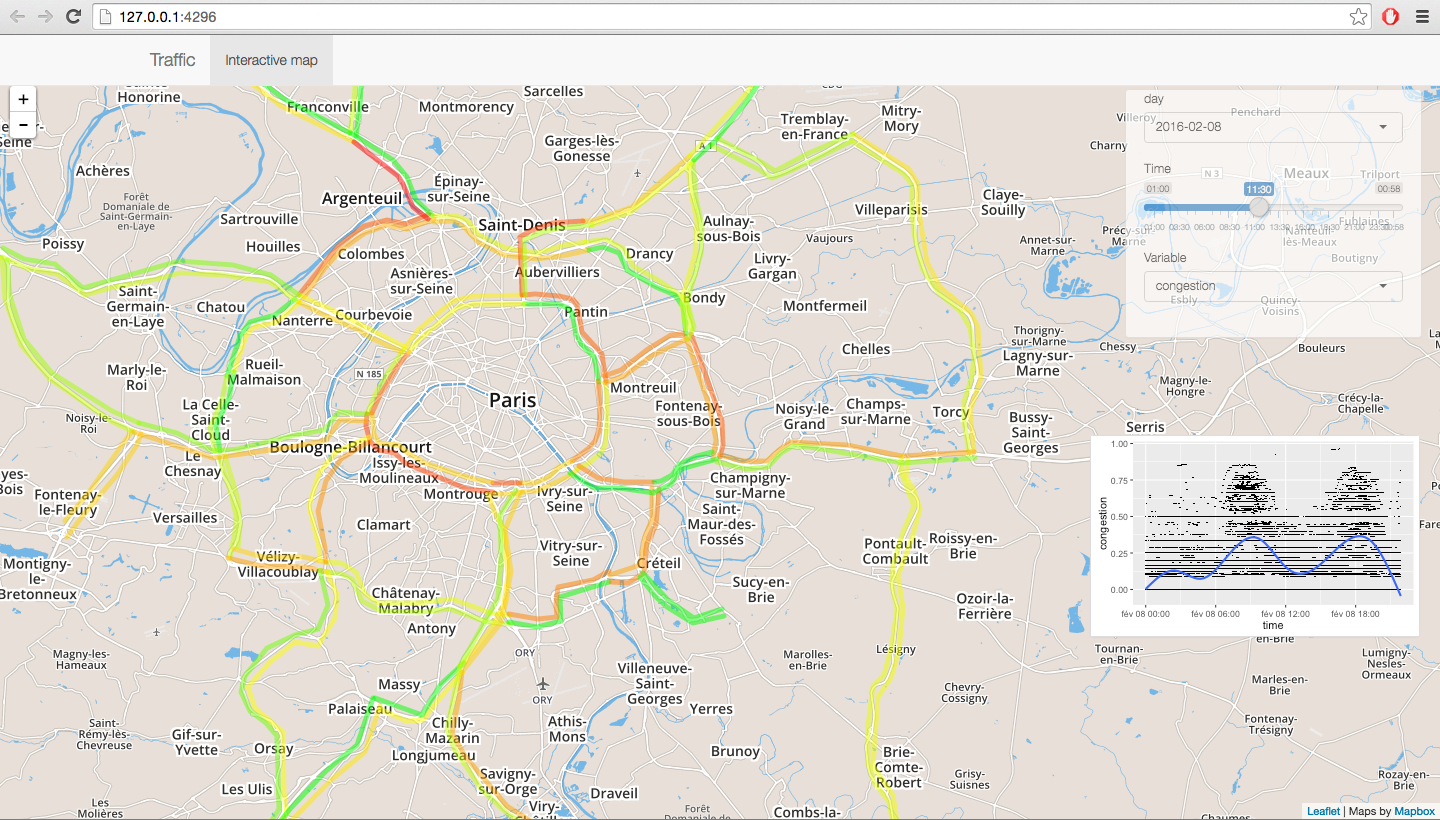
\includegraphics[width=\linewidth]{Figures/TransportationEquilibrium/gr1}
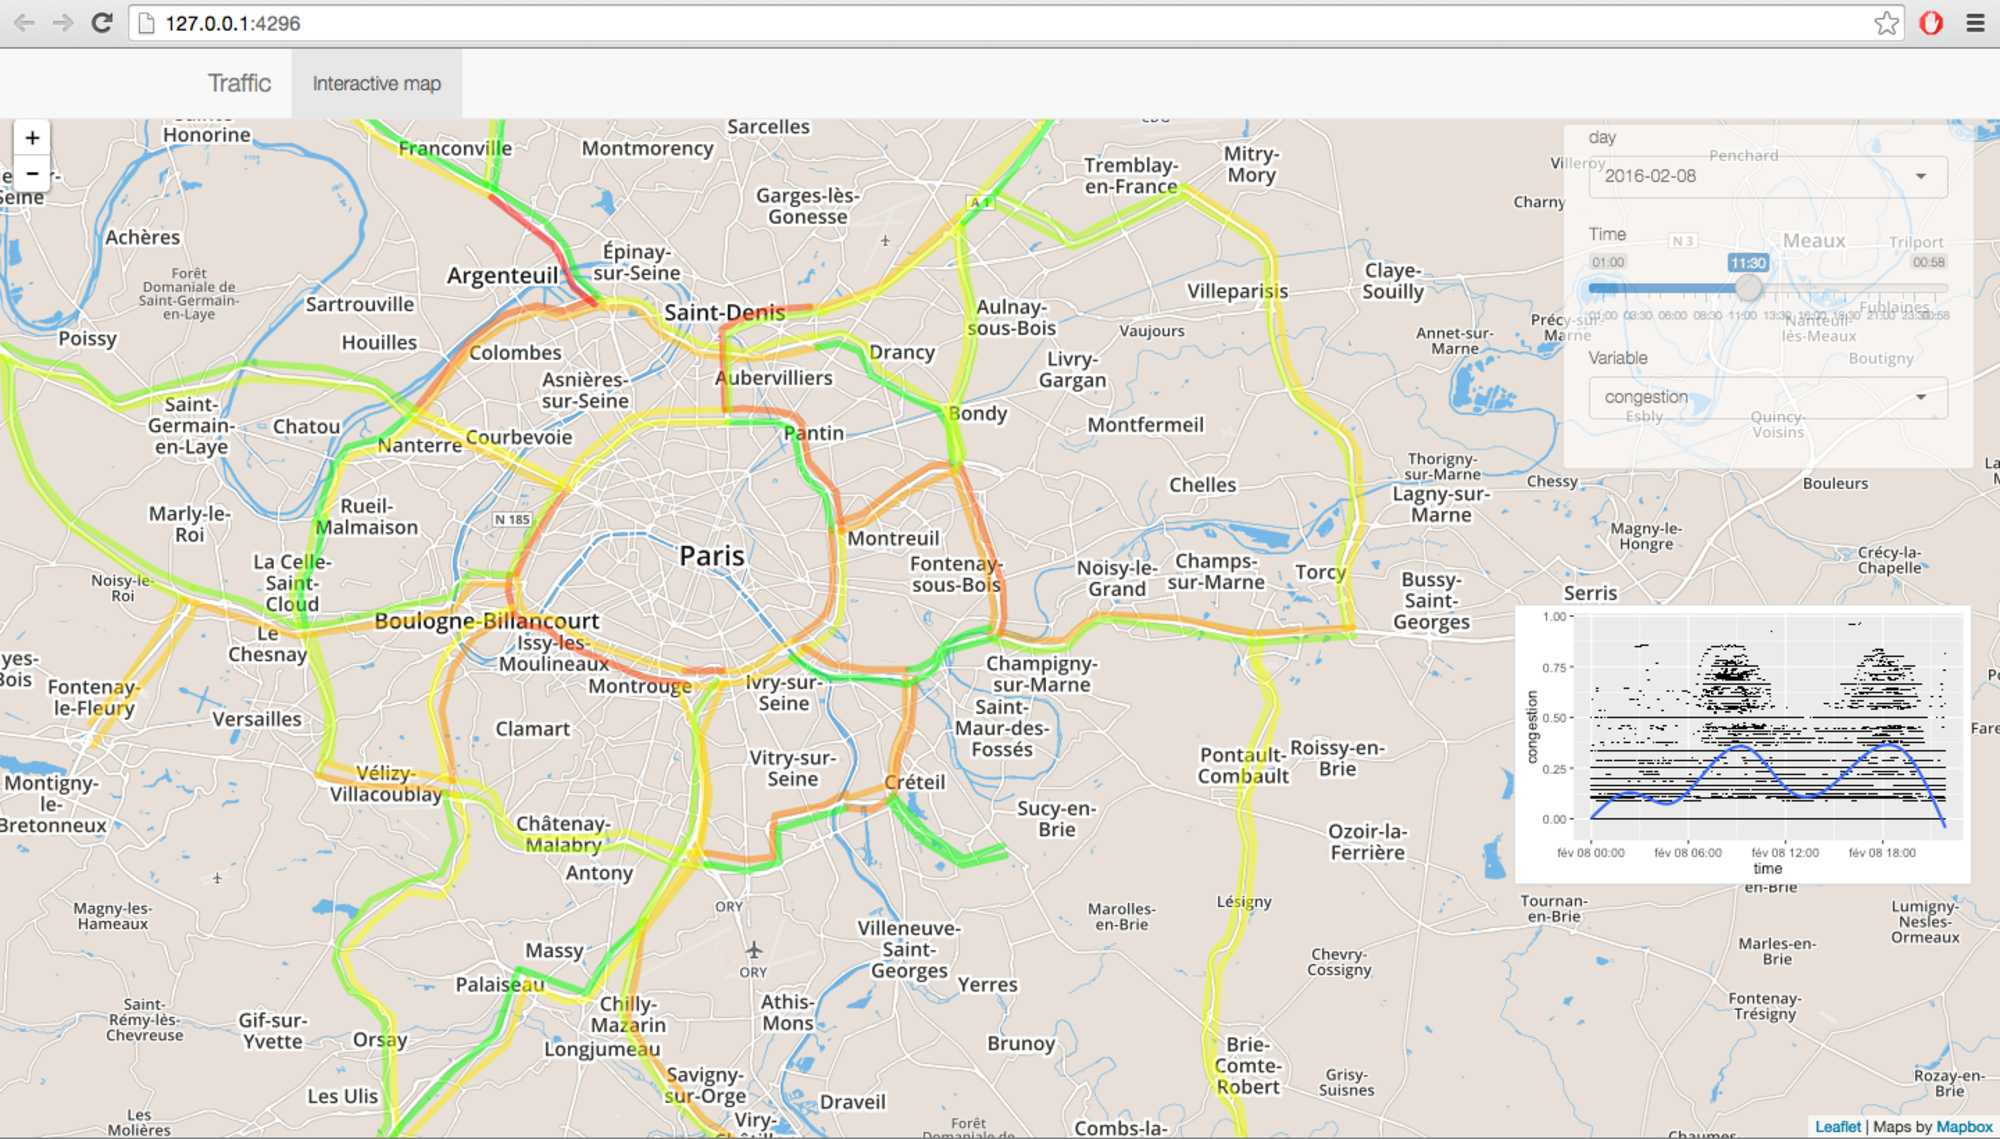
\includegraphics[width=\linewidth]{Figures/Final/8-1-2-fig-transportationequilibrium-fig-1.jpg}
\caption[Web-application for traffic data][Application web pour les données de trafic]{Capture of the web-application to explore spatio-temporal traffic data for Parisian region. It is possible to select date and time (precision of 15min on one month, reduced from initial dataset for performance purposes). A plot summarizes congestion patterns on the current day.\label{fig:transportationequilibrium:fig-1}}{Capture de l'application web\comment[FL]{developpee par/pour (?) qui ?} permettant l'exploration spatio-temporelle des données de traffic pour la région Parisienne. Il est possible de choisir date et heure (précision de 15min sur un mois, réduite par rapport au jeu de données initial pour des raisons de performance). Le graphe en insert résume les motifs de congestion pour la journée courante, en donnant en fonction du temps l'ensemble des valeurs (points noirs) et leur lissage (courbe bleue).\label{fig:transportationequilibrium:fig-1}}
\end{figure}
%%%%%%%%%%%%%%%%%%



%%%%%%%%%%%%%%%%%%%%%%%%
\paragraph{Spatio-temporal Variability of Travel Path}{Variabilité Spatio-temporelle des Trajets}


\bpar{
Following interactive exploration of data, we propose to quantify the spatial variability of congestion patterns to validate or invalidate the intuition that if equilibrium does exist in time, it is strongly dependent on space and localized. The variability in time and space of travel-time shortest paths is a first way to investigate flow stationarities from a game-theoretic point of view. Indeed, the static User Equilibrium is the stationary distribution of flows under which no user can improve its travel time by changing its route. A strong spatial variability of shortest paths at short time scales is thus evidence of non-stationarity, since a similar user will take a few time after a totally different route and not contribute to the same flow as a previous user. Such a variability is indeed observed on a non-negligible number of paths on each day of the dataset. We show in Figure~\ref{fig:fig-2} an example of extreme spatial variation of shortest path for a particular Origin-Destination pair.
}{
A la suite de l'exploration interactive des données, nous proposons de quantifier la variabilité spatiale des motifs de congestion pour valider ou invalider l'intuition que si l'équilibre existe par rapport au temps, il est fortement dépendant de l'espace et localisé. La variabilité spatio-temporelle des plus courts chemins de trajet est une première façon d'étudier la stationnarité des flots d'un point de vue de théorie des jeux. En effet, l'Equilibre Utilisateur Statique est la distribution stationnaire des flots sous laquelle aucun utilisateur ne peut augmenter son temps de trajet en changeant son itinéraire. Une forte variabilité spatiale des plus courts chemins sur de courtes échelles spatiales révèle ainsi une non-stationnarité, puisque un même utilisateur prendra un chemin complètement différent après un court laps de temps et ne contribuera plus au même flot que précédemment. Une telle variabilité est en effet observée sur un nombre non-négligeable de chemins pour chaque jour du jeu de données. La figure~\ref{fig:fig-2} montre un exemple de variation spatiale extrême d'un trajet pour une paire Origine-Destination particulière.
}

\bpar{
The systematic exploration of travel time variability across the whole dataset, and associated travel distance, confirms, as described in Figure 3, that travel time absolute variability has often high values of its maximum across OD pairs, up to 25 minutes with a temporal local mean around 10min. Corresponding spatial variability produces detours up to 35km.
}{
L'exploration systématique de la variabilité du temps de trajet sur l'ensemble du jeu de données, et des distances de trajet associées, confirme, comme présenté en figure~\label{fig:fig-3}, que la variation absolue du temps de trajet présente fréquemment une forte variation de son maximum sur l'ensemble des paires O-D, jusqu'à 25 minutes avec une moyenne temporelle locale autour de 10 minutes. La variabilité spatiale correspondante entraine des détours allant jusqu'à 35km.
}


%%%%%%%%%%%%%%%%%%%
\begin{figure}
%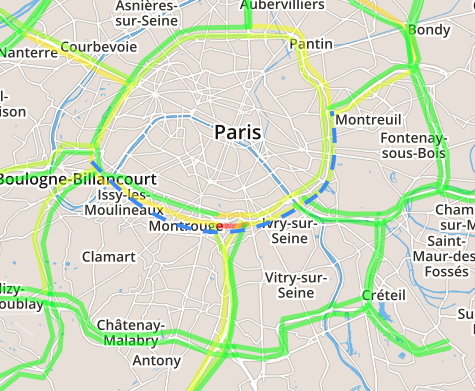
\includegraphics[width=0.47\linewidth]{Figures/TransportationEquilibrium/gr21}
%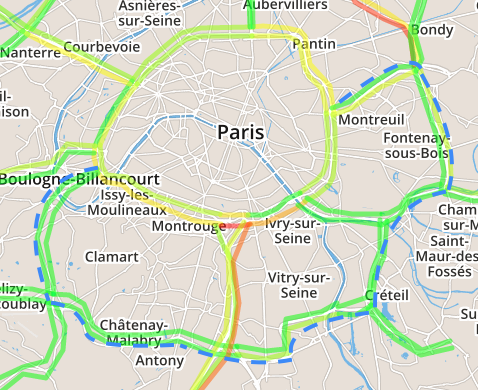
\includegraphics[width=0.47\linewidth]{Figures/TransportationEquilibrium/gr22}
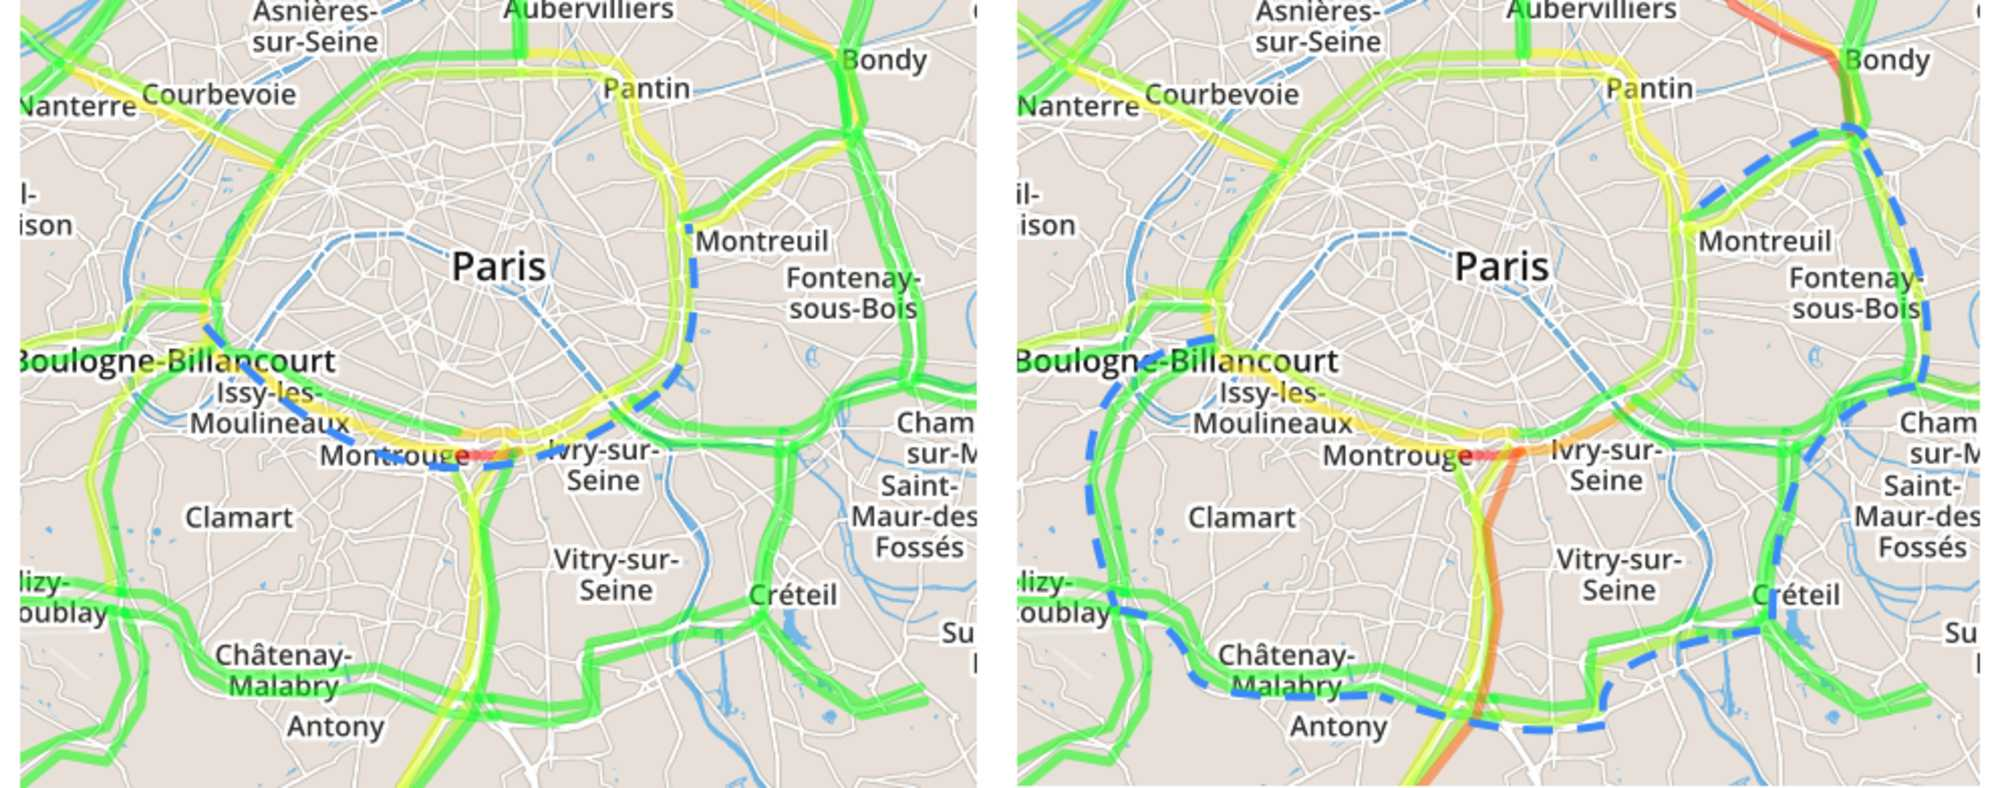
\includegraphics[width=\linewidth]{Figures/Final/8-1-2-fig-transportationequilibrium-fig-2.jpg}
\caption[Spatial variability of shortest paths][Variabilité spatiale des plus courts chemins]{Spatial variability of travel-time shortest path (shortest path trajectory in dotted blue). In an interval of only 10 minutes, between 11/02/2016 00:06 (left) and 11/02/2016 00:16 (right), the shortest path between \emph{Porte d'Auteuil} (West) and \emph{Porte de Bagnolet} (East), increases in effective distance of $\simeq 37$km (with an increase in travel time of only 6min), due to a strong disruption on the ring of Paris.\label{fig:fig-2}}{Variabilité spatiale d'un plus court chemin en temps de trajet (trajet du plus court chemin en pointillé bleu). Dans un intervalle de seulement 10 minutes, entre le 11/02/2016 00:06 (à gauche) et le 11/02/2016 00:16 (à droite), le plus court chemin entre Porte d'Auteuil à l'ouest et Porte de Bagnolet à l'est, augmente en distance effective de $\simeq 37$km (avec une augmentation du temps de trajet de seulement 6 minutes), à cause d'une forte perturbation sur le périphérique parisien.\label{fig:transportationequilibrium:fig-2}}
\end{figure}
%%%%%%%%%%%%%%%%%%%



%%%%%%%%%%%%%%%%%%%
\begin{figure}
%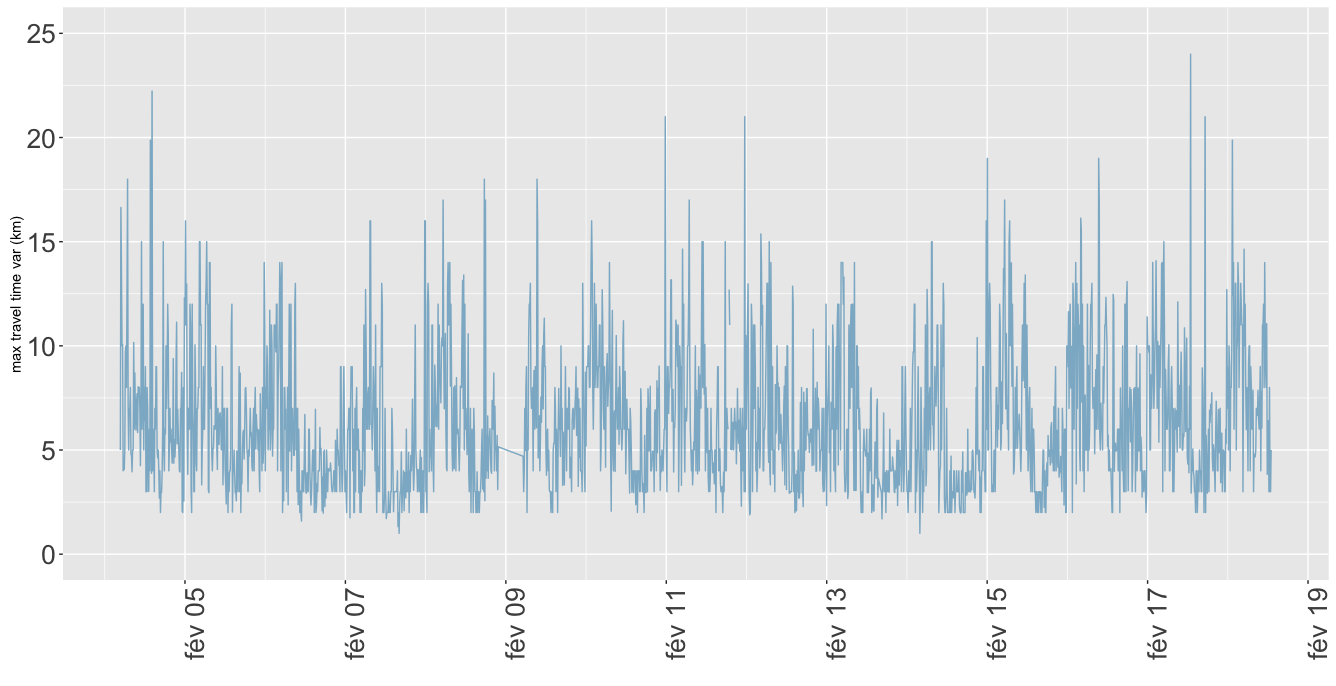
\includegraphics[width=\linewidth]{Figures/TransportationEquilibrium/gr31}
%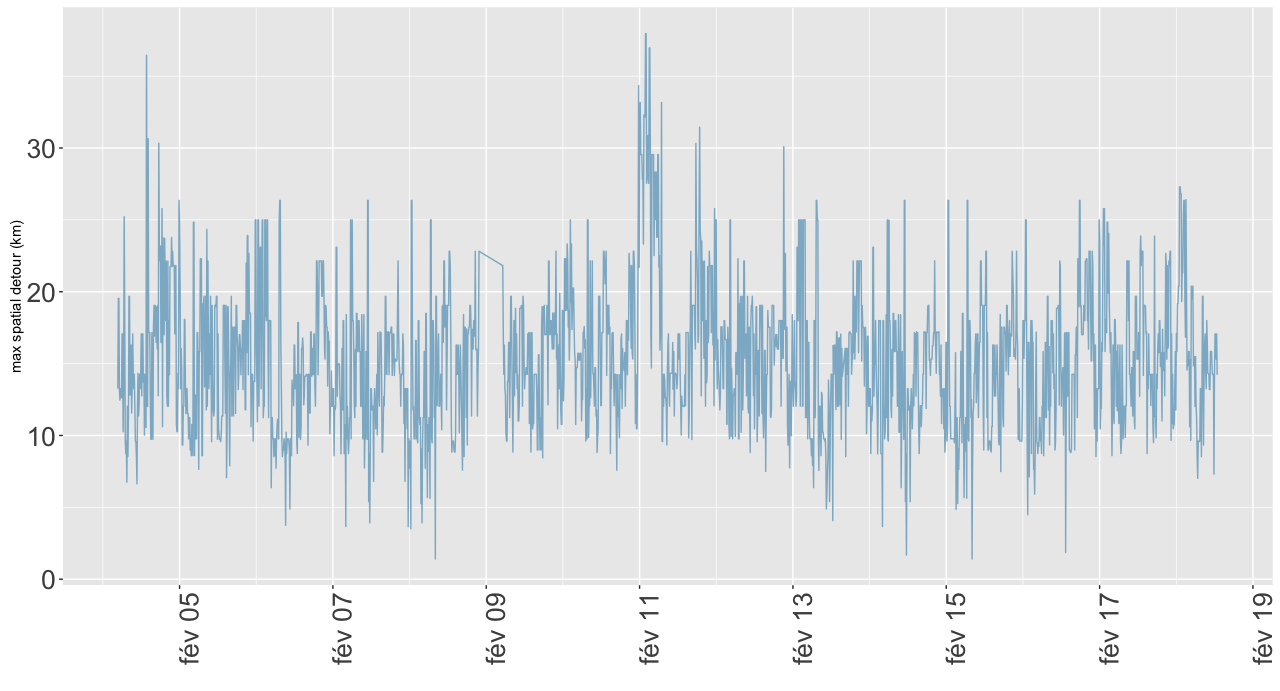
\includegraphics[width=\linewidth]{Figures/TransportationEquilibrium/gr32}
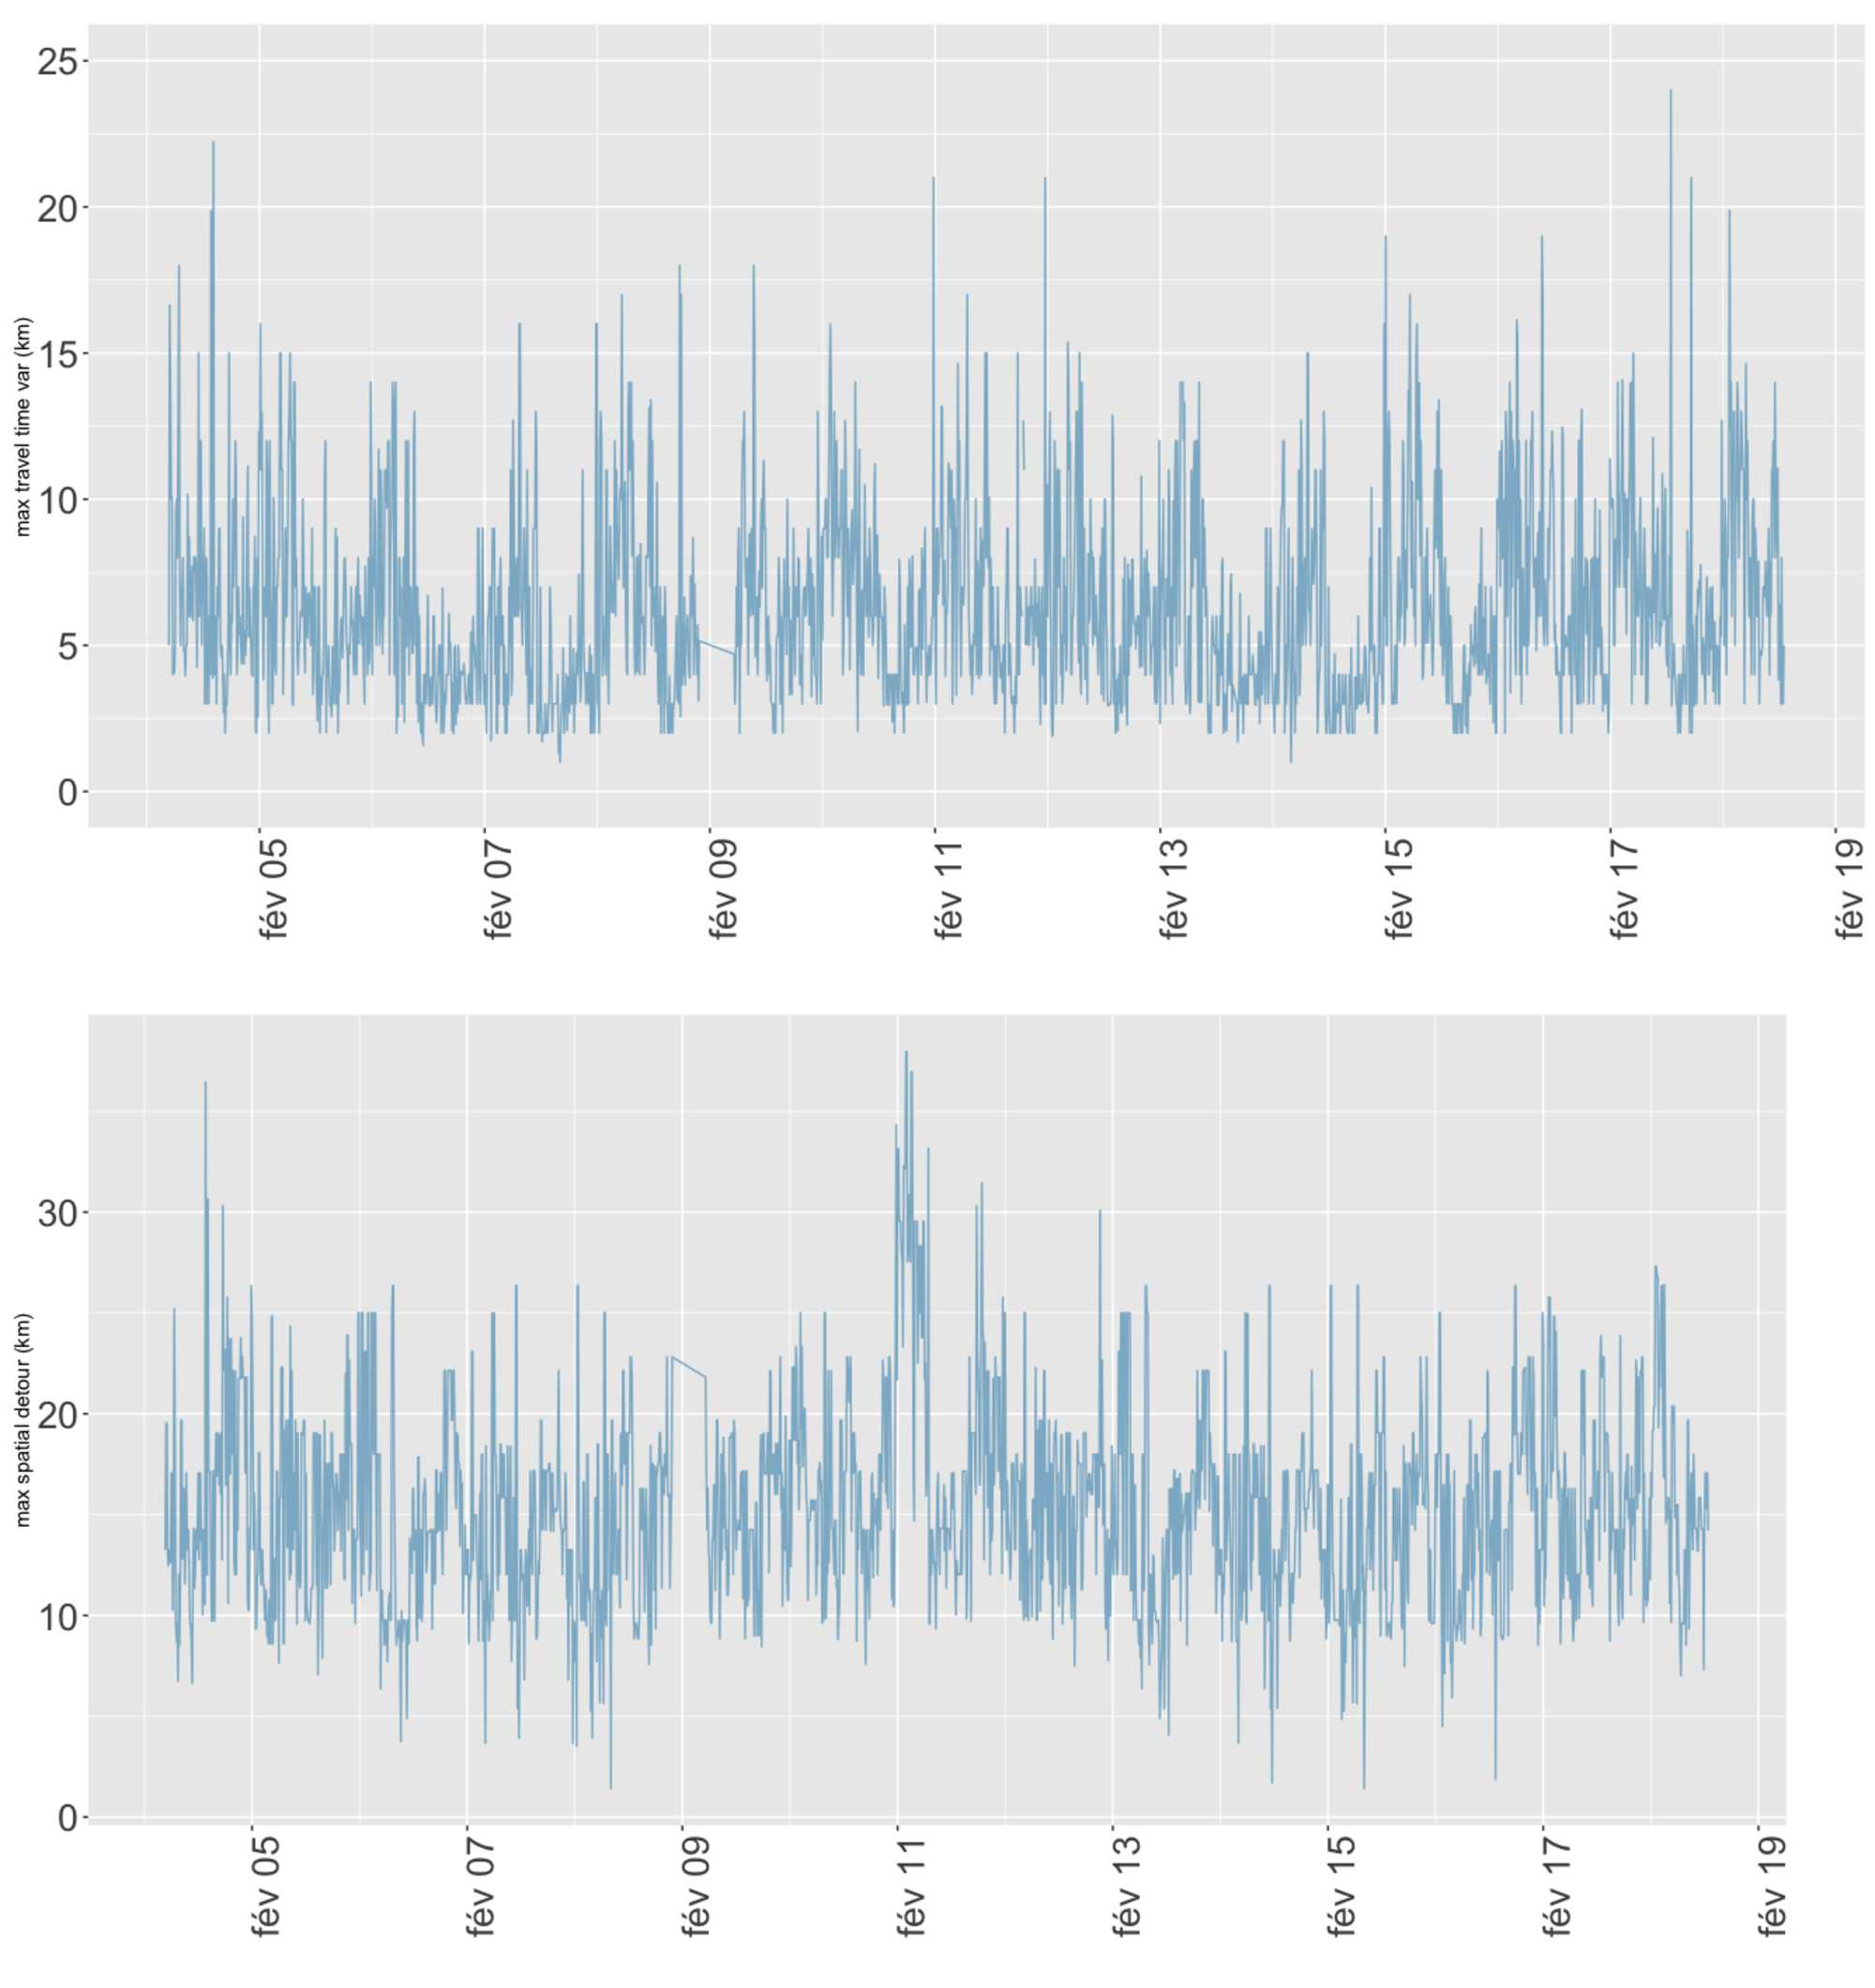
\includegraphics[width=\linewidth]{Figures/Final/8-1-2-fig-transportationequilibrium-fig-3.jpg}
\caption[Variability of travel time and distance][Variabilité des temps de trajet]{Travel time (top) in min and corresponding travel distance (bottom) maximal variability on a two weeks sample. We plot the maximal on all OD pairs of the absolute variability between two consecutive time steps. Peak hours imply a high time travel variability up to 25 minutes and a path length variability up to 35km.\label{fig:transportationequilibrium:fig-3}}{Variabilité maximale du temps de trajet (en haut) en minutes et de la distance de trajet correspondante (en bas) pour un échantillon de deux semaines. Le graphe représente le maximum sur l'ensemble des paires Origine-Destination de la variabilité absolue entre deux pas de temps consécutifs. Les heures de pointe induisent une forte variabilité du temps de trajet, allant jusqu'à 25 minutes et une variabilité de distance jusqu'à 35km.\label{fig:transportationequilibrium:fig-3}\comment[FL]{pourquoi le choix de cet indicateur ? par ex. si le detour correspond a une OD tres tres minoritaire, en quoi est-ce pertinent ?}[(JR) j'avais rajouté cet indicateur pour répondre à une remarque d'un reviewer, mais en effet il casse pas des briques. il faut faire une hypothèse que vu qu'on a une granularité assez grande, la plupart des OD seront réalisés (de plus en prenant les sous-trajets).]}
\end{figure}
%%%%%%%%%%%%%%%%%%%




%%%%%%%%%%%%%%%%%%%
\paragraph{Stability of Network measures}{Stabilité des mesures de réseau}

\bpar{
The variability of potential trajectories observed in the previous section can be confirmed by studying the variability of network properties. In particular, network topological measures capture global patterns of a transportation network. Centrality and node connectivity measures are classical indicators in transportation network description as recalled in~\cite{bavoux2005geographie}. The transportation literature has developed elaborated and operational network measures, such as network robustness measures to identify critical links and measure overall network resilience to disruptions (an example among many is the Network Trip Robustness index introduced in~\cite{sullivan2010identifying}).
}{
La variabilité des trajectoires potentielles observée dans la section précédente peu être confirmée par l'étude de la variabilité des propriétés du réseau. En particulier, les mesures topologiques de réseau capturent les motifs globaux dans un réseau de transport. Les mesures de centralité et de connectivité des noeuds sont des indicateurs classiques pour la description des réseaux de transport comme rappelé par~\cite{bavoux2005geographie}. La littérature en transports a développé des mesures de réseau élaborées et opérationnelles, comme des mesures de robustesse pour identifier les liens critiques et mesurer la résilience globale du réseau aux perturbations (un exemple parmi d'autres est l'indice de \emph{Robustesse du Réseau Effective} introduit dans ~\cite{sullivan2010identifying}).
}



\bpar{
More precisely, we study the betweenness centrality of the transportation network, defined for a node as the number of shortest paths going through the node, i.e. by the equation

%%%%%%%%%%%%%%%
% equation betweeness
\begin{equation}
b_i = \frac{1}{N(N-1)}\cdot \sum_{o\neq d \in V}\mathbbm{1}_{i\in p(o\rightarrow d)}
\end{equation}
%%%%%%%%%%%%%%%

where $V$ is the set of network vertices of size $N$, and $p(o\rightarrow d)$ is the set of nodes on the shortest path between vertices o and d (the shortest path being computed with effective travel times). This index is more relevant to our purpose than other measures of centrality such as closeness centrality that does not include potential congestion as betweenness centrality does.
}{
Plus précisément, nous étudions la centralité de chemin du réseau de transport, défini pour un noeud comme le nombre de plus courts chemins passant par celui-ci, i.e. par l'équation

%%%%%%%%%%%%%%%
% equation betweeness
\begin{equation}
b_i = \frac{1}{N(N-1)}\cdot \sum_{o\neq d \in V}\mathbbm{1}_{i\in p(o\rightarrow d)}
\end{equation}
%%%%%%%%%%%%%%%

où $V$ est l'ensemble des sommets du réseau de taille $N$, et $p(o\rightarrow d)$ est l'ensemble des noeuds sur le plus court chemin entre les sommets $o$ et $d$ (le plus court chemin étant calculé avec le temps de trajet effectif). Cette mesure de centralité est plus adaptée que d'autre dans notre cas, comme la centralité de proximité qui n'inclut pas la congestion potentielle comme la centralité de chemin.
}



\bpar{
We show in Figure 4 the relative absolute variation of maximal betweenness centrality for the same time window than previous empirical indicators. More precisely we plot the value of

%%%%%%%%%%%%%%%
% eq relative variability
\begin{equation}
\Delta b(t) = \frac{\left|\max_i (b_i(t + \Delta t)) - \max_i (b_i(t))\right|}{\max_i (b_i(t))}
\end{equation}
%%%%%%%%%%%%%%%



where $\Delta t$ is the time step of the dataset (the smallest time window on which we can capture variability). This absolute relative variation has a direct meaning : a variation of 20\% (which is attained a significant number of times as shown in Fig.~\ref{fig:fig-4}) means that in case of a negative variation, at least this proportion of potential travels have changed route and the local potential congestion has decrease of the same proportion. In the case of a positive variation, a single node has captured at least 20\% of travels. Under the assumption (that we do not try to verify in this work and assume to be also not verified as shown by~\cite{zhu2010people}, but that we use as a tool to give an idea of the concrete meaning of betweenness variability) that users rationally take the shortest path and assuming that a majority of travels are realized such a variation in centrality imply a similar variation in effective flows, leading to the conclusion that they can not be stationary in time (at least at a scale larger than $\Delta t$) nor in space.
}{
Nous montrons en Fig.~\ref{fig:transportationequilibrium:fig-4} la variation relative absolue du maximum de la centralité de chemin, pour la même fenêtre temporelle que les indicateurs empiriques précédents. Plus précisément, elle est définie par


%%%%%%%%%%%%%%%
% eq relative variability
\begin{equation}
\Delta b(t) = \frac{\left|\max_i (b_i(t + \Delta t)) - \max_i (b_i(t))\right|}{\max_i (b_i(t))}
\end{equation}
%%%%%%%%%%%%%%%


où $\Delta t$ est le pas de temps du jeu de données (la plus petite fenêtre temporelle sur laquelle une variabilité peut être capturée). Cette variation relative absolue a une signification directe : une variation de 20\% (qui est atteinte un nombre significatif de fois comme montré en Figure~\ref{fig:transportationequilibrium:fig-4}) implique dans le cas d'une variation négative, qu'au moins cette proportion de trajectoires potentielles ont changé et que la potentielle congestion locale a décru de la même proportion. Dans le cas d'une variation positive, un seul noeud a capturé au moins 20\% des trajets. Sous l'hypothèse (qu'on ne tente pas de vérifier ici et qu'on peut également supposer non vérifiée comme montré par~\cite{zhu2010people}, mais que l'on utilise comme un outil pour donnée une intuition sur la signification concrète de la variabilité de la centralité) que les utilisateurs choisissent rationnellement le plus court chemin, et supposant que la majorité des trajets est réalisées, une telle variation de la centralité implique une variation similaire dans les flots effectifs, conduisant à la conclusion qu'ils ne peuvent être stationnaires ni dans le temps (au moins sur une échelle plus grande que $\Delta t$) ni dans l'espace.
}




%%%%%%%%%%%%%%%%%%%
\begin{figure}
%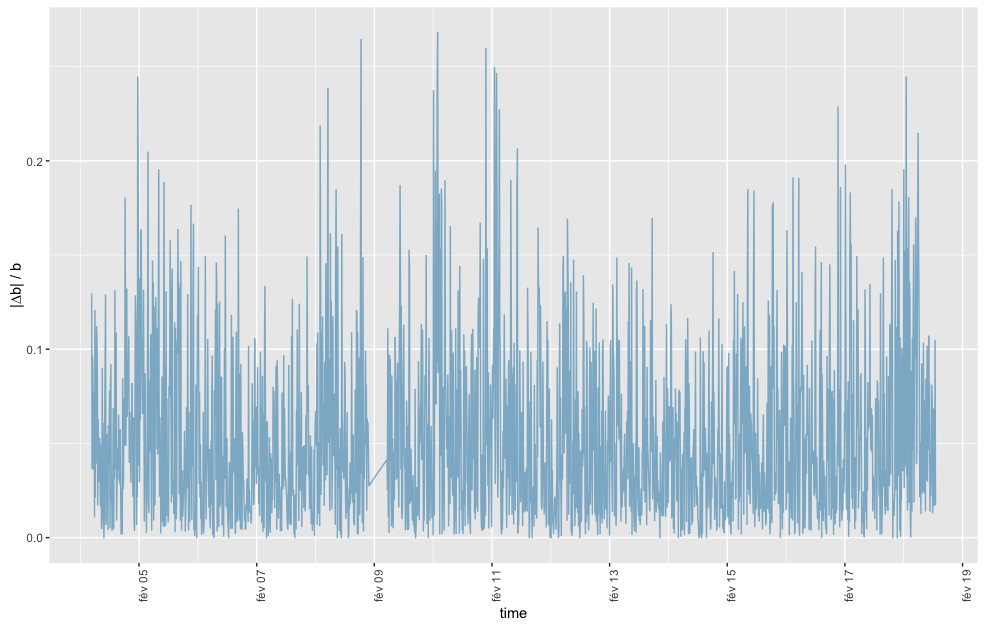
\includegraphics[width=\linewidth]{Figures/TransportationEquilibrium/gr4}
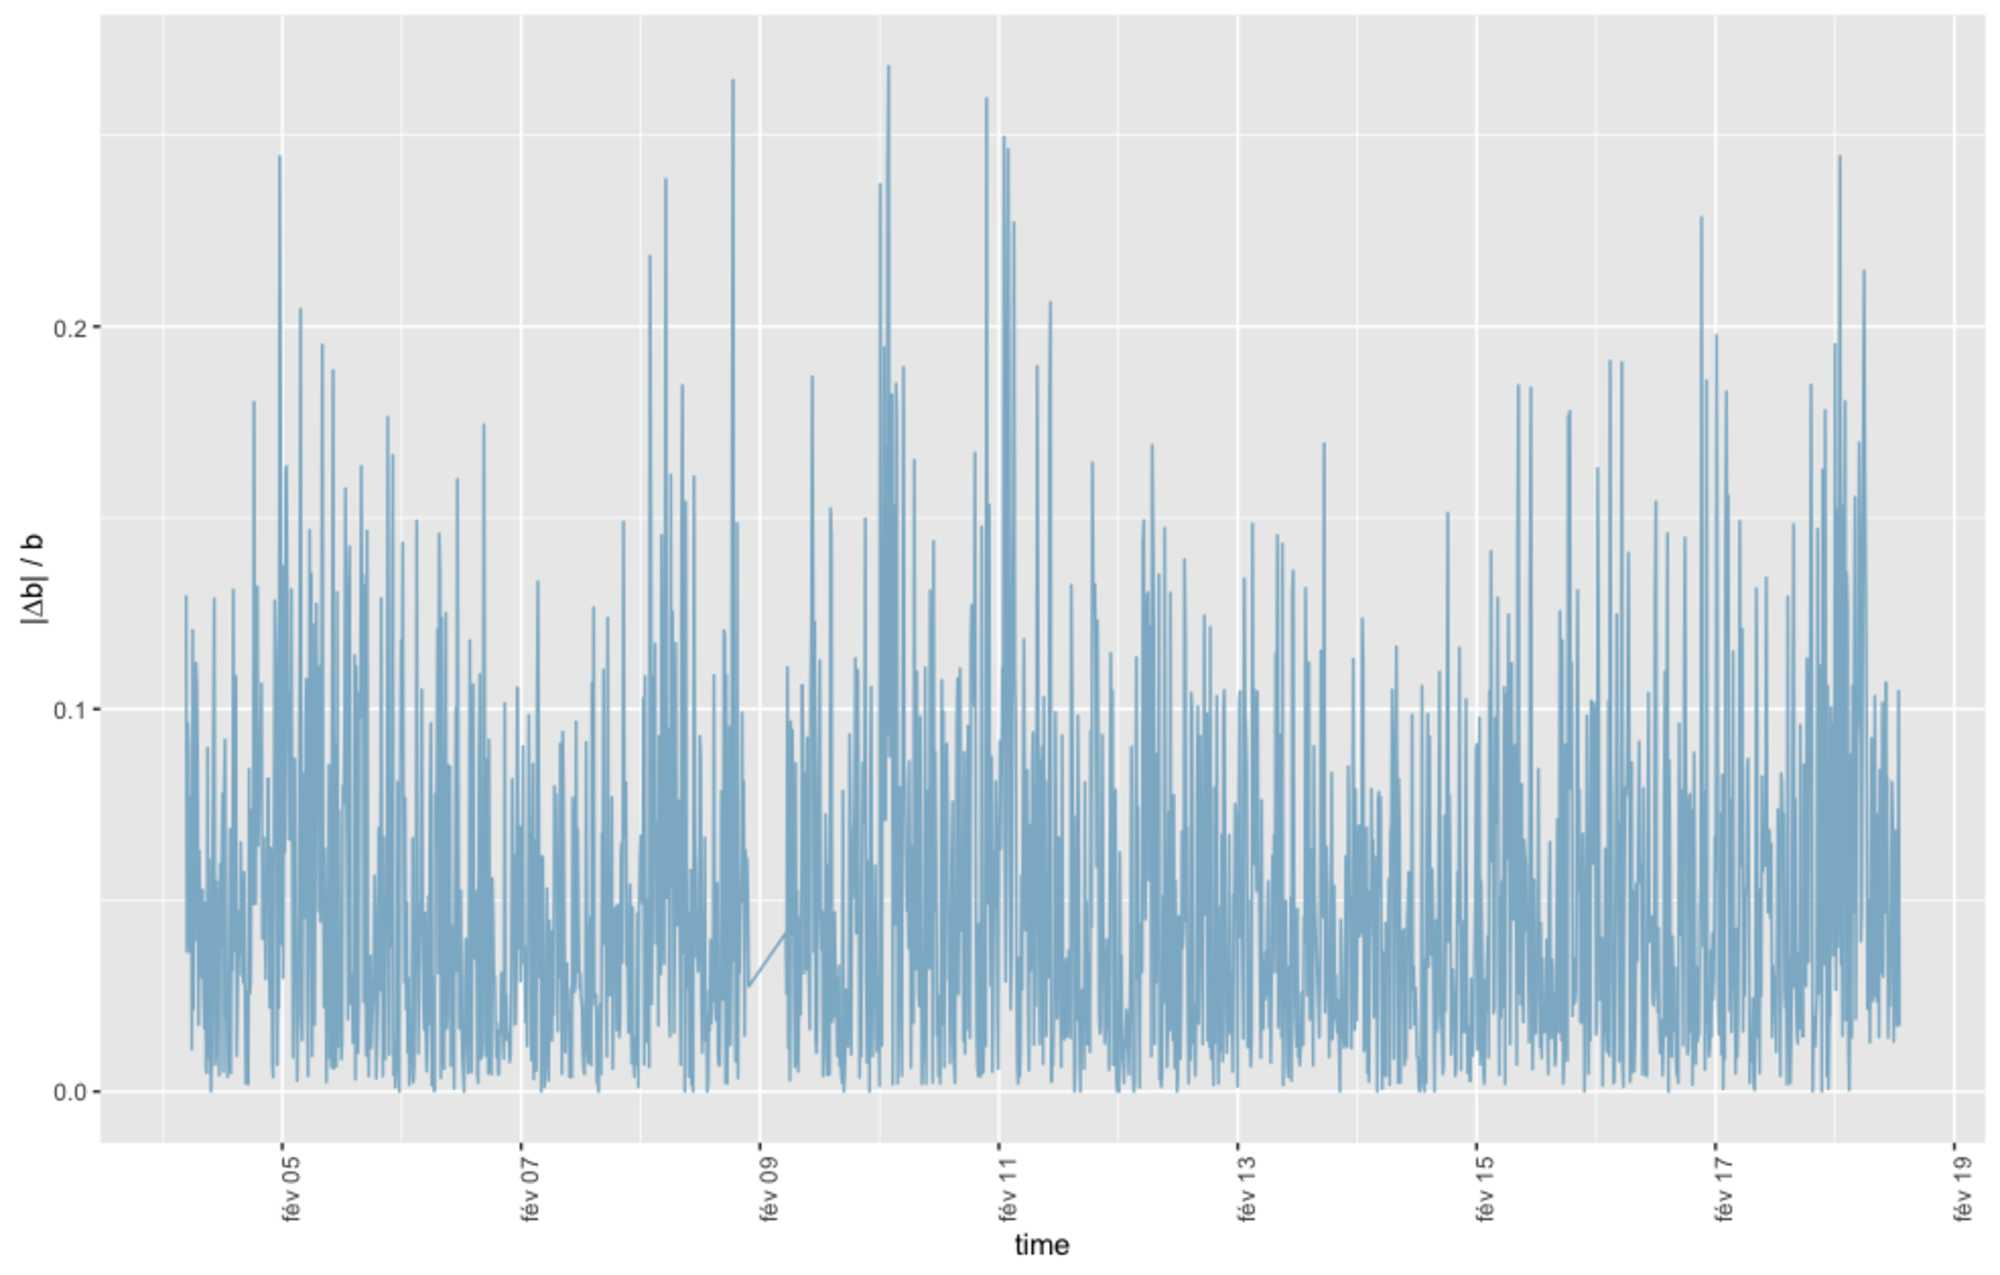
\includegraphics[width=\linewidth]{Figures/Final/8-1-2-fig-transportationequilibrium-fig-4.jpg}
\caption[Temporal stability of maximal betweenness centrality][Stabilité temporelle de la centralité]{Temporal stability of maximal betweenness centrality. We plot in time the normalized derivative of maximal betweenness centrality, that expresses its relative variations at each time step. The maximal value up to 25\% correspond to very strong network disruption on the concerned link, as it means that at least this proportion of travelers assumed to take this link in previous conditions should take a totally different path.\label{fig:transportationequilibrium:fig-4}}{Stabilité temporelle du maximum de la centralité de chemin. Le graphe montre dans le temps la dérivée normalisée du maximum de la centralité de chemin, qui capture ses variations relatives à chaque pas de temps. La valeur maximale de 25\% correspond à de très fortes perturbations du réseau sur les liens correspondants, puisque cela implique qu'au moins cette proportion d'utilisateurs prenant le lien dans des conditions précédentes doivent prendre un trajet complètement différent.\label{fig:transportationequilibrium:fig-4}\comment[FL]{ce n'est pas possible a lire $\rightarrow$ synthetiser}[(JR) pas pertinent de lisser, car c'est justement les max locaux qui nous intéressent.]}
\end{figure}
%%%%%%%%%%%%%%%%%%%





%%%%%%%%%%%%%%%%%%%
\paragraph{Spatial heterogeneity of equilibrium}{Hétérogénéité spatiale de l'équilibre}



\bpar{
To obtain a different insight into spatial variability of congestion patterns, we propose to use an index of spatial autocorrelation, the Moran index (defined e.g. in~\cite{tsai2005quantifying}). More generally used in spatial analysis with diverse applications from the study of urban form to the quantification of segregation, it can be applied to any spatial variable. It allows to establish neighborhood relations and unveils spatial local consistence of an equilibrium if applied on localized traffic variable. At a given point in space, local autocorrelation for variable c is computed by

%%%%%%%%%%%%
% Moran index def
\begin{equation}
\rho_i = \frac{1}{K}\cdot \sum_{i\neq j}{w_{ij}\cdot (c_i - \bar{c})(c_j - \bar{c})}
\end{equation}
%%%%%%%%%%%%

where $K$ is a normalization constant equal to the sum of spatial weights times variable variance and $\bar{c}$ is variable mean. In our case, we take spatial weights of the form $w_{ij} = \exp{\left(\frac{-d_{ij}}{d_0}\right)}$ with $d_0$ typical decay distance and compute the autocorrelation of link congestion localized at link center. We capture therefore spatial correlations within a radius of same order than decay distance around the point $i$. The mean on all points yields spatial autocorrelation index $I$. A stationarity in flows should yield some temporal stability of the index.
}{
Afin d'obtenir un point de vue différent sur la variabilité spatiale des motifs de congestion, nous proposons d'utiliser un indice d'auto-corrélation spatiale, l'indice de Moran (défini par exemple dans~\cite{tsai2005quantifying}). Utilisé plus généralement en analyse spatiale, avec diverses applications allant de l'étude de la forme urbaine à la quantification de la ségrégation, il peut être appliqué à toute variable spatiale. Il permet d'établir des relations de voisinage et révèle la consistence spatiale locale d'un équilibre s'il est appliqué à une variable de traffic localisée. A un point donnée de l'espace, l'auto-corrélation locale pour la variable $c$ est calculée par

%%%%%%%%%%%%
% Moran index def
\begin{equation}
\rho_i = \frac{1}{K}\cdot \sum_{i\neq j}{w_{ij}\cdot (c_i - \bar{c})(c_j - \bar{c})}
\end{equation}
%%%%%%%%%%%%

où $K$ est une constante de normalisation égale à la somme des poids spatiaux fois la variance de la variable et $\bar{c}$ est la moyenne de la variable. Dans notre cas, nous choisissons des poids spatiaux de la forme $w_{ij} = \exp{\left(\frac{-d_{ij}}{d_0}\right)}$ avec $d_0$ distance typique de décroissance. L'auto-corrélation est calculée sur la congestion des liens, localisée au centre du lien. Elle capture ainsi les corrélations spatiales dans un rayon du même ordre que la distance de décroissance autour du point $i$. La moyenne sur l'ensemble des points fournit l'indice d'auto-corrélation spatiale $I$. Une stationnarité des flots devrait impliquer une stabilité temporelle de l'index. 
}



\bpar{
Figure~\ref{fig:transportationequilibrium:fig-5} presents temporal evolution of spatial autocorrelation for congestion. As expected, we have a strong decrease of autocorrelation with distance decay parameter, for both amplitude and temporal average. The high temporal variability implies short time scales for potential stationarity windows. When comparing with congestion (fitted to plot scale for readability) for 1km decay, we observe that high correlations coincide with off-peak hours, whereas peaks involve vanishing correlations. Our interpretation, combined with the observed variability of spatial patterns, is that peak hours correspond to chaotic behaviour of the system, as jams can emerge in any link: correlation thus vanishes as feasible phase space for a chaotic dynamical system is filled by trajectories in an uniform way what is equivalent to apparently independent random relative speeds.
}{
La figure~\ref{fig:transportationequilibrium:fig-5} présente l'évolution temporelle de l'auto-corrélation spatiale pour la congestion. Comme attendu, on observe une forte décroissance de l'auto-corrélation avec la distance de décroissance, à la fois sur l'amplitude et les moyennes temporelles. La forte variabilité temporelle implique de courtes échelles temporelles pour des fenêtres potentielles de stationnarité. Pour une distance de décroissance de 1km, en comparant l'auto-corrélation à la congestion (ajustée à l'échelle du graphe pour lisibilité), on observe que les fortes corrélations coincident avec les heures creuses, tandis que les heures de pointe correspondent à une décroissance des corrélations. Notre interprétation, combinée avec la variabilité observée des motifs spatiaux, est que les heures de pointe correspondent à un comportement chaotique du système, puisque les bouchons peuvent émerger dans n'importe quel lien du réseau : la corrélation disparait alors puisque l'espace des phases atteignables pour un système dynamique chaotique est rempli uniformément par les trajectoires, de façon équivalente à des vitesses relatives qui apparaitraient comme aléatoires et indépendantes.
}



%%%%%%%%%%%%%%%%
\begin{figure}
%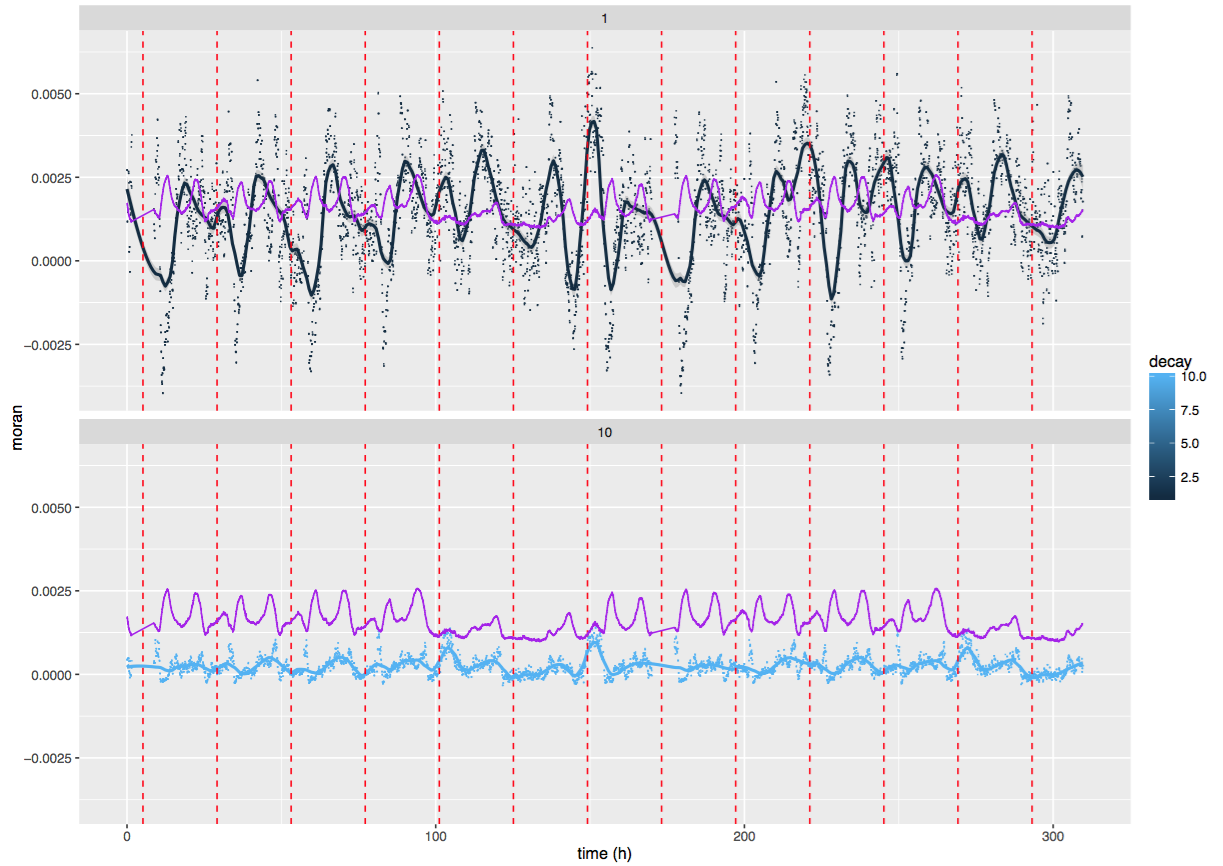
\includegraphics[width=\linewidth]{Figures/TransportationEquilibrium/gr5}
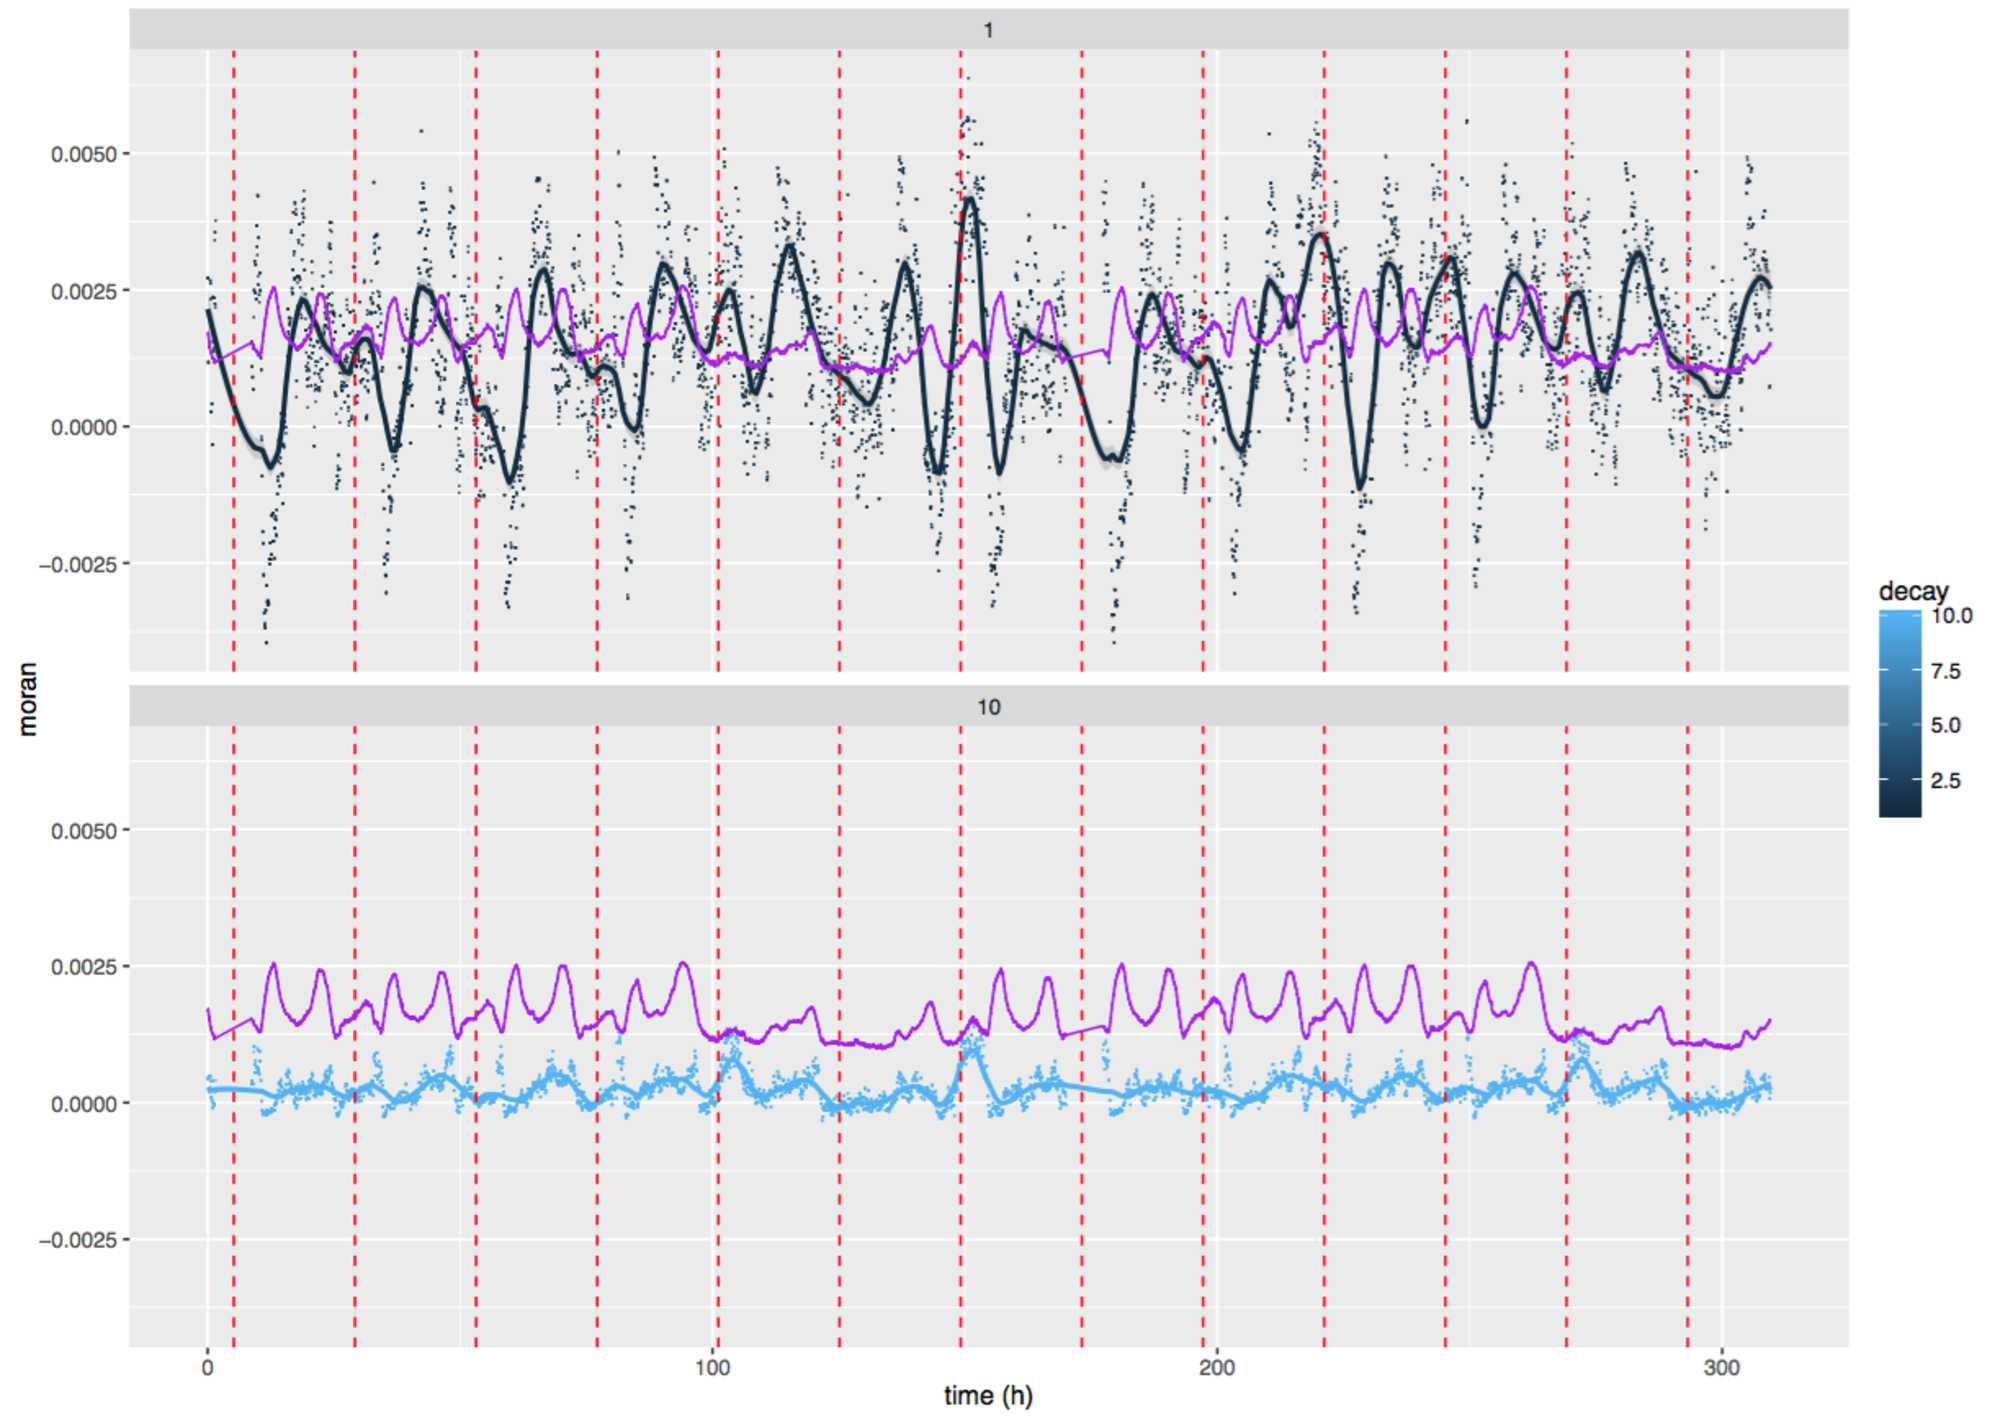
\includegraphics[width=\linewidth]{Figures/Final/8-1-2-fig-transportationequilibrium-fig-5.jpg}
\caption[Spatial auto-correlations for relative travel speed][Auto-corrélation spatiale]{Spatial auto-correlations for relative travel speed on two weeks. We plot for varying value of decay parameter (1,10km) values of auto-correlation index in time. Intermediate values of decay parameter yield a rather continuous deformation between the two curves. Points are smoothed with a 2h span to ease reading. Vertical dotted lines correspond to midnight each day. Purple curve is relative speed fitted at scale to have a correspondence between auto-correlation variations and peak hours.\label{fig:transportationequilibrium:fig-5}}{Auto-corrélations spatiales pour les vitesses relatives sur deux semaines. Le graphe montre les valeurs de l'auto-corrélation dans le temps, pour des valeurs variables (1,10km) de la distance de décroissance. les valeurs intermédiaires de la distance de décroissance donnent une déformation relativement continue entre ces deux extrêmes. Les points sont lissés sur une fenêtre temporelle de 2h pour faciliter la lecture. Les lignes pointillées verticales correspondent à minuit de chaque jour. La courbe violette donne la vitesse relative, ajustée à l'échelle pour établir la correspondance entre les heures de pointe et les variations de l'auto-corrélation.\label{fig:transportationequilibrium:fig-5}}
\end{figure}
%%%%%%%%%%%%%%%%




%%%%%%%%%%%%%%%%%%%%
\subsection{Discussion}{Discussion}

\subsubsection{Theoretical and practical implications of empirical conclusions}{Implications théoriques et pratiques des conclusions empiriques}

\bpar{
We argue that the theoretical implications of our empirical findings do not imply in a total discarding of the Static User Equilibrium framework, but unveil more a need of stronger connections between theoretical literature and empirical studies. If each newly introduced theoretical framework is generally tested on one on more case study, there are no systematic comparisons of each on large and different datasets and on various objectives (prediction of traffic, reproduction of stylized facts, etc.) as systematic reviews are the rule in therapeutic evaluation for example. This imply however broader data and model sharing practices than the current ones. The precise knowledge of application potentialities for a given framework may induce unexpected developments such as its integration into larger models. The example of Land-use and Transportation Interaction studies (LUTI models) is a good illustration of how the SUE can still be used for larger purpose than transportation modeling. \cite{kryvobokov2013comparison} describe two LUTI models, one of which includes two equilibria for four-step transportation model and for land-use evolution (households and firms relocation), the other being more dynamical. The conclusion is that each model has its own advantages regarding the pursued objective, and that the static model can be used for long time policy purposes, whereas the dynamic model provide more precise information at smaller time scale. In the first case, a more complicated transportation module would have been complicated to include, what is an advantage of the static user equilibrium.
}{
Nous formulons l'interprétation que les implications théoriques de ces résultats empiriques n'impliquent pas nécessairement un rejet total du cadre de l'Equilibre Utilisateur Statique, mais révèlent plutôt un besoin de plus fortes connexions entre la littérature théorique et les études empiriques. Si chaque nouveau cadre théorique introduit est généralement testé sur un cas ou plus, il n'existe pas de comparaisons systématiques de chacun sur des jeux de données de grande taille et variés, et pour des objectifs d'application différents (prédiction du traffic, reproduction de faits stylisés, etc.), à l'image des revues systématiques qui sont la règle en évaluation thérapeutique par exemple.\comment[FL]{source ?} Cela implique cependant des pratiques de partage des données et des modèles plus larges que celles existant couramment. La connaissance précise des potentialités d'application d'un cadre donné peut induire des développements inattendus comme l'intégration dans des modèles plus larges. L'exemple des études des interaction entre Transport et Usage du Sol (modèles \emph{LUTI}) est une bonne illustration d'un cas ou le EUS peut toujours être utilisé avec des motivations plus larges que la modélisation du traffic. \cite{kryvobokov2013comparison} décrit deux modèles \emph{LUTI}, dont l'un inclut deux équilibres pour les modèles de transport à quatre temps et pour l'évolution de l'usage du sol (localisation des ménages et emplois), l'autre étant dynamique. La conclusion est que chaque modèle à ses avantages au regard de l'objectif poursuivi, et que le modèle statique peut être utilisé pour comparer des politiques sur le temps long, tandis que le modèle dynamique fournit de l'information plus précise à de plus petites échelles temporelles. Dans le premier cas, un module de transport plus compliqué aurait été plus difficile à inclure, ce qui est un avantage du EUS dans ce cas.
}


\bpar{
Concerning practical applications, it seems natural that static models should not be used for traffic forecast and management at small time scales (week or day) and efforts should be made to implement more realistic models. However the use of models by the planning and engineering community is not necessarily directly related to academic concerns and state-of-the-art. For the particular case of France and mobility models, \cite{commenges2013invention} showed that engineers had gone to the point of constructing inexistent problems and implementing corresponding models that they had imported from a totally different geographical context (planning in the United States). The use of one framework or type of model has historical reasons that may be difficult to overcome.
}{
Concernant les applications pratiques, il semble naturel\comment[FL]{je ne pense pas que tu as prouve cela : tu ne dis pas comment sont utilises ces modeles} que les modèles statiques ne devraient pas être utilisés pour la prédiction et la gestion du traffic sur de petites échelles temporelles (semaine ou jour) et que des efforts doivent être faits pour implémenter des modèles plus réalistes. Cependant, l'utilisation des modèles par la communautés des ingénieurs et des planificateurs n'est pas directement reliée aux enjeux académiques et à l'état de l'art dans le domaine. Dans le cas particulier de la France et des modèles de mobilité, \cite{commenges2013invention} a montré que les ingénieurs allaient jusqu'au point de construire des problèmes inexistants et d'implémenter les modèles correspondants qu'ils avaient importé d'un contexte géographique totalement différent (la planification aux Etats-Unis). L'utilisation d'un cadre ou d'un type de modèle a des raisons historiques qui peuvent être difficiles à surmonter.

}


\subsubsection{Towards explanative interpretations of non-stationarity}{Vers des interprétations de la non-stationnarité}


\bpar{
An assumption we formulate regarding the origin of non-stationarity of network flows, in view of data exploration and quantitative analysis of the database, is that the network is at least half of the time highly congested and in a critical state. The off-peak hours are the larger potential time windows of spatial and temporal stationarity, but consist in less than half of the time. As already interpreted through the behavior of autocorrelation indicator, a chaotic behavior may be at the origin of such variability in the congested hours. The same way a supercritical fluid may condense under the smallest external perturbation, the state of the link may qualitatively change with a small incident, producing a network disruption that may propagate and even amplify. The direct effect of traffic events (notified incidents or accidents) can not be studied without external data, and it could be interesting to enrich the database in that direction. It would allow establishing the proportion of disruptions that do appear to have a direct effect and quantify a level of criticality of network congestion in time, or to investigate more precise effects such as the consequences of an incident on traffic of the opposite lane.
}{
Une hypothèse qu'on peut formuler concernant l'origine de la non-stationnarité des flots dans le réseau, au regard de l'exploration des données et des analyses quantitatives, est que le réseau est au moins la moitié du temps fortement congestionné et dans un état critique. Les heures creuses sont les plus grandes fenêtres temporelles potentielles de stationnarité spatiale et temporelle, mais couvre moins de la moitié du temps. Comme déjà interprété dans le comportement de l'indicateur d'auto-corrélation, un comportement chaotique pourrait être à l'origine d'une telle variabilité lors des heures congestionnées. A la manière d'un fluide supercritique qui condense sous une perturbation externe infinitésimale, l'état d'un lien peut qualitativement changer par un petit incident, produisant une perturbation du réseau qui se propage et peut même s'amplifier. L'effet direct des évènements du traffic (incidents signalés ou accidents) ne peut pas être étudié sans source de données extérieure, et un enrichissement de la base de données dans cette direction pourrait être intéressante. Cela permettrait d'établir la proportion de perturbations qui paraissent avoir un effet direct et quantifier un niveau de caractère critique de la congestion du réseau dans le temps, ou d'étudier plus précisément des phénomènes localisés comme les conséquences d'un incident de traffic sur la voie opposée.
}



\subsubsection{Possible developments}{Développements}


\bpar{
Further work may be planned towards a more refined assessment of temporal stability on a region of the network, i.e. the quantitative investigation of consideration of peak stationarity given above. To do so we propose to compute numerically Liapounov stability of the dynamical system ruling traffic flows using numerical algorithms such as described by~\cite{goldhirsch1987stability}. The value of Liapounov exponents provides the time scale by which the unstable system runs out of equilibrium. Its comparison with peak duration and average travel time, across different spatial regions and scales should provide more information on the possible validity of the local stationarity assumption. This technique has already been introduced at an other scale in transportation studies, as e.g.~\cite{tordeux2016jam} that study the stability of speed regulation models at the microscopic scale to avoid traffic jams.
}{
Le travail futur pourra être planifié dans la direction d'une étude de la stabilité temporelle sur des zones du réseau, i.e. l'étude quantitative précise de la non-stationnarité des heures de pointes découverte ci-dessus. Pour cela nous proposons de calculer numériquement la stabilité de Liapounov du système dynamique régissant les flots de traffic, par l'intermédiaire d'algorithmes numériques comme ceux décrits par~\cite{goldhirsch1987stability}. La valeur des exposants de Liapounov fournit l'échelle de temps sur laquelle le système instable s'éloigne de l'équilibre. Leur comparaison avec la durée des heures de pointe et le temps de trajet moyen, sur différentes zones spatiales et différentes échelles, devrait fournir plus d'information sur une possible validité de l'hypothèse de stationnarité locale. Cette technique a déjà été introduite à une autre échelle dans les études de transport, comme e.g.~\cite{tordeux2016jam} qui étudie la stabilité des modèles de régulation de vitesse à l'échelle microscopique pour éviter l'émergence de congestion.
}


\bpar{
Other research directions may consist in the test of other assumptions of static user equilibrium (as the rational shortest path choice, which would be however difficult to test on such an aggregated dataset, implying the use of simulation models calibrated and cross-validated on the dataset to compare assumptions, without necessarily a direct clear validation or invalidation of the assumption), or the empirical computation of parameters in stochastic or dynamical user equilibrium frameworks. 
}{
D'autres directions de recherche peuvent consister en le test des autres hypothèses du EUS (comme le choix rationnel du plus court chemin, qui serait cependant difficile à tester à un tel niveau d'agrégation, impliquant l'utilisation de modèles de simulation calibrés et cross-validés sur le jeu de données pour comparer différentes hypothèses, sans toutefois nécessairement une validation ou invalidation directe de l'hypothèse), ou le calcul empirique des paramètres dans les cadres d'Equilibre Utilisateur Stochastique ou Dynamique.
}



\subsubsection{Conclusion}{Conclusion}


\bpar{
We have described an empirical study aimed at a simple but from our point of view necessary investigation of the existence of the static user equilibrium, more precisely of its stationarity in space and time on a metropolitan highway network. We constructed by data collection a traffic congestion dataset for the highway network of Greater Paris on 3 months with two minutes temporal granularity. The interactive exploration of the dataset with a web application allowing spatio-temporal data visualization helped to guide quantitative studies. Spatio-temporal variability of shortest paths and of network topology, in particular betweenness centrality, revealed that stationarity assumptions do not hold in general, what was confirmed by the study of spatial autocorrelation of network congestion. We suggest that our findings highlight a general need of higher connections between theoretical and empirical studies, as our work can discard misunderstandings on the theoretical static user equilibrium framework and guide the choice of potential applications.
}{
Nous avons décrit une étude empirique ayant pour but une étude simple, mais selon notre point de vue nécéssaire, de l'existence de l'équilibre utilisateur statique, plus précisément de sa stationnarité dans le temps et l'espace pour un réseau routier métropolitain principal. Un jeu de données de congestion du trafic est construite par collection de données, pour le réseau du Grand Paris sur 3 mois avec une granularité temporelle de 2 minutes. L'exploration interactive du jeu de données via une application web permettant la visualisation spatio-temporelle aide à guider les analyses quantitatives. La variabilité spatio-temporelle des plus courts chemins et de la topologie du réseau, en particulier la centralité de chemin, révèle que l'hypothèse de stationnarité ne tient généralement pas, ce qui est confirmé par l'étude de l'auto-corrélation spatiale de la congestion du réseau. Nous suggérons que nos résultats soulignent un besoin général de plus grandes connexions entre les études théoriques et empiriques, puisque cette étude permet de chasser les incompréhensions théoriques sur l'Equilibre Utilisateur Statique, et guider le choix d'application potentielles.
}



\stars




